\section{LIONESS wide-block cipher scheme}
\label{appendix:lioness}

HOPR uses the LIONESS \cite{lionesspaper} wide-block cipher scheme with ChaCha20 as stream cipher and BLAKE2s as hash function, resulting in a key length of 128 bytes and 64 bytes for the initialisation vector.

The key $k$ is split into four chunks of 32 bytes $k = k_1 \ || \ k_2 \ || \  k_3 \ || \ k_4$, where $k_1, k_3$ are used as keys for the stream cipher and $k_2, k_4$ are used to key the hash function. The same applies to the initialisation vector $iv$ which is split into four chunks of 16 bytes $iv = iv_1 \ || \ iv_2 \ || \  iv_3 \ || \ iv_4$ with $iv_1, iv_3$ as an initialisation vector for the stream cipher and $iv_2, iv_4$ as an initialisation vector for the hash function.

\begin{figure}[H]
    \centering
    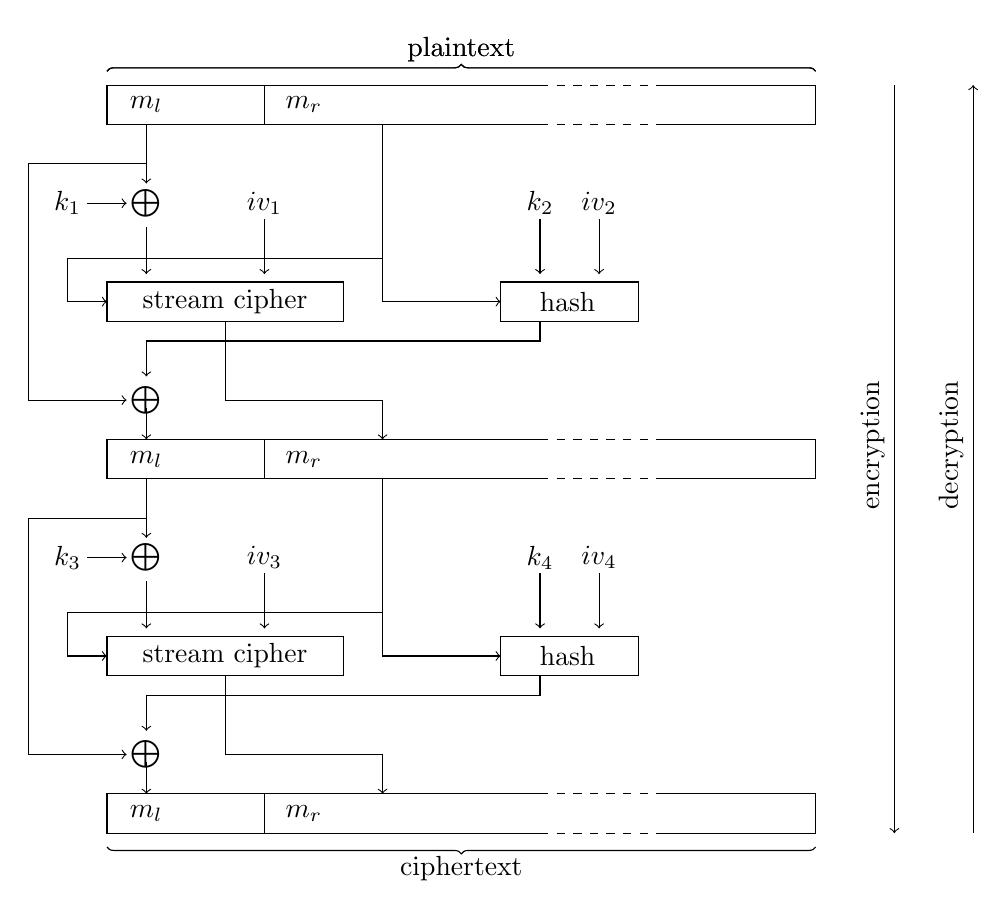
\begin{tikzpicture}
        \def\hashLength{2}
        \def\cipherLength{7}
        \def\messageOffset{3.5}
        \def\messageOffsetWidth{1.5}

        \draw[->] (\hashLength+\cipherLength+1,0.5) -- node[above=5pt,rotate=90] {encryption} (\hashLength+\cipherLength+1,-9.0);

        \draw[->] (\hashLength+\cipherLength+2,-9.0) -- node[above=5pt,rotate=90] {decryption} (\hashLength+\cipherLength+2,0.5);

        \draw[decoration={brace,raise=5pt},decorate] (0,0.5) -- node[above=5pt] {plaintext} (\hashLength+\cipherLength,0.5);


        \draw[decoration={brace,raise=5pt},decorate] (0,0.5) -- node[above=5pt] {plaintext} (\hashLength+\cipherLength,0.5);

        \foreach \i\j\offset in{1/2/0,3/4/-4.5} {
                \begin{scope}[shift={(0,\offset)}]
                    \draw (0,0) rectangle (\hashLength,0.5);
                    \draw (\hashLength+\messageOffset,0.5) -- (\hashLength, 0.5) -- (\hashLength, 0.0) -- (\hashLength+\messageOffset,0.0);
                    \draw (\hashLength+\messageOffset+\messageOffsetWidth,0.5) -- (\hashLength+\cipherLength, 0.5) -- (\hashLength+\cipherLength,0.0) -- (\hashLength+\messageOffset+\messageOffsetWidth,0.0);
                    \draw [dashed] (\hashLength+\messageOffset,0.5) -- (\hashLength+\messageOffset+\messageOffsetWidth,0.5) (\hashLength+\messageOffset,0.0) -- (\hashLength+\messageOffset+\messageOffsetWidth,0.0);

                    \draw (0.5,0.25) node {$m_l$};
                    \draw (\hashLength+0.5,0.25) node {$m_r$};

                    % Encryption
                    \draw (0.5,-1) node {$\bigoplus$};
                    \draw (-0.5,-1) node {$k_\i$};
                    \draw (2,-1) node {$iv_\i$};

                    \draw [->] (0.5,0) -- (0.5,-0.75);
                    \draw [->] (-0.25,-1) -- (0.25,-1);
                    \draw [->] (0.5,-1.3) -- (0.5,-1.9);
                    \draw [->] (2,-1.2) -- (2,-1.9);

                    \draw (0,-2.5) rectangle (3, -2);
                    \draw (1.5, -2.25) node [align=center] {stream cipher};

                    % into stream cipher
                    \draw [->] (\hashLength+1.5, 0) -- (\hashLength+1.5, -1.7) -- (-0.5,-1.7) -- (-0.5,-2.25) -- (0,-2.25);

                    \draw [->] (1.5,-2.5) -- (1.5,-3.5) -- (\hashLength+1.5,-3.5) -- (\hashLength+1.5,-4);

                    %Hashing
                    \draw (5.5,-1) node {$k_\j$};
                    \draw (6.25,-1) node {$iv_\j$};

                    \draw [->] (5.5,-1.2) -- (5.5,-1.9);
                    \draw [->] (6.25,-1.2) -- (6.25,-1.9);

                    \draw (5,-2.5) rectangle (6.75, -2);
                    \draw (5.85, -2.25) node [align=center] {hash};

                    \draw [->] (5.5,-2.5) -- (5.5, -2.75) -- (0.5,-2.75) -- (0.5,-3.2);
                    \draw (0.5,-3.5) node {$\bigoplus$};

                    \draw [->] (0.5,-0.5) -- (-1,-0.5) -- (-1,-3.5) -- (0.25,-3.5);
                    \draw [->] (0.5, -3.6) -- (0.5, -4);

                    %m_r into hash
                    \draw [->] (\hashLength+1.5,-1.7) -- (\hashLength+1.5, -2.25) -- (5,-2.25);
                \end{scope}
            }

        \begin{scope}[shift={(0,-9.0)}]
            \draw (0,0) rectangle (\hashLength,0.5);
            \draw (\hashLength+\messageOffset,0.5) -- (\hashLength, 0.5) -- (\hashLength, 0.0) -- (\hashLength+\messageOffset,0.0);
            \draw (\hashLength+\messageOffset+\messageOffsetWidth,0.5) -- (\hashLength+\cipherLength, 0.5) -- (\hashLength+\cipherLength,0.0) -- (\hashLength+\messageOffset+\messageOffsetWidth,0.0);
            \draw [dashed] (\hashLength+\messageOffset,0.5) -- (\hashLength+\messageOffset+\messageOffsetWidth,0.5) (\hashLength+\messageOffset,0.0) -- (\hashLength+\messageOffset+\messageOffsetWidth,0.0);

            \draw (0.5,0.25) node {$m_l$};
            \draw (\hashLength+0.5,0.25) node {$m_r$};
        \end{scope}

        \draw[decoration={brace,raise=5pt,mirror},decorate] (0,-9.0) -- node[below=5pt] {ciphertext} (\hashLength+\cipherLength,-9.0);


    \end{tikzpicture}
    \caption{Schematic overview of encryption and decryption of the LIONESS \cite{lionesspaper} scheme}
\end{figure}

LIONESS is an unbalanced Feistel scheme, hence decryption is achieved by applying the operations used for encryption in the inverse order. In contrast to other Feistel schemes, the plaintext $m$ is not split equally and the size of the parts depend on the output length of used hash function.

As HOPR payloads have a size of 500 bytes, messages are split as $m = m_l \ || \ m_r$ where $|m_l| = 32$ bytes and $|m_r| = 468$ bytes.